\documentclass[border=10pt]{standalone}

\usepackage{tikz}
\usepackage{tikzsymbols}
\usetikzlibrary{calc,patterns,shapes.geometric}

\def\centerarc[#1](#2)(#3:#4:#5){\draw[#1] ($(#2)+({#5*cos(#3)},{#5*sin(#3)})$) arc (#3:#4:#5);}

\begin{document}
	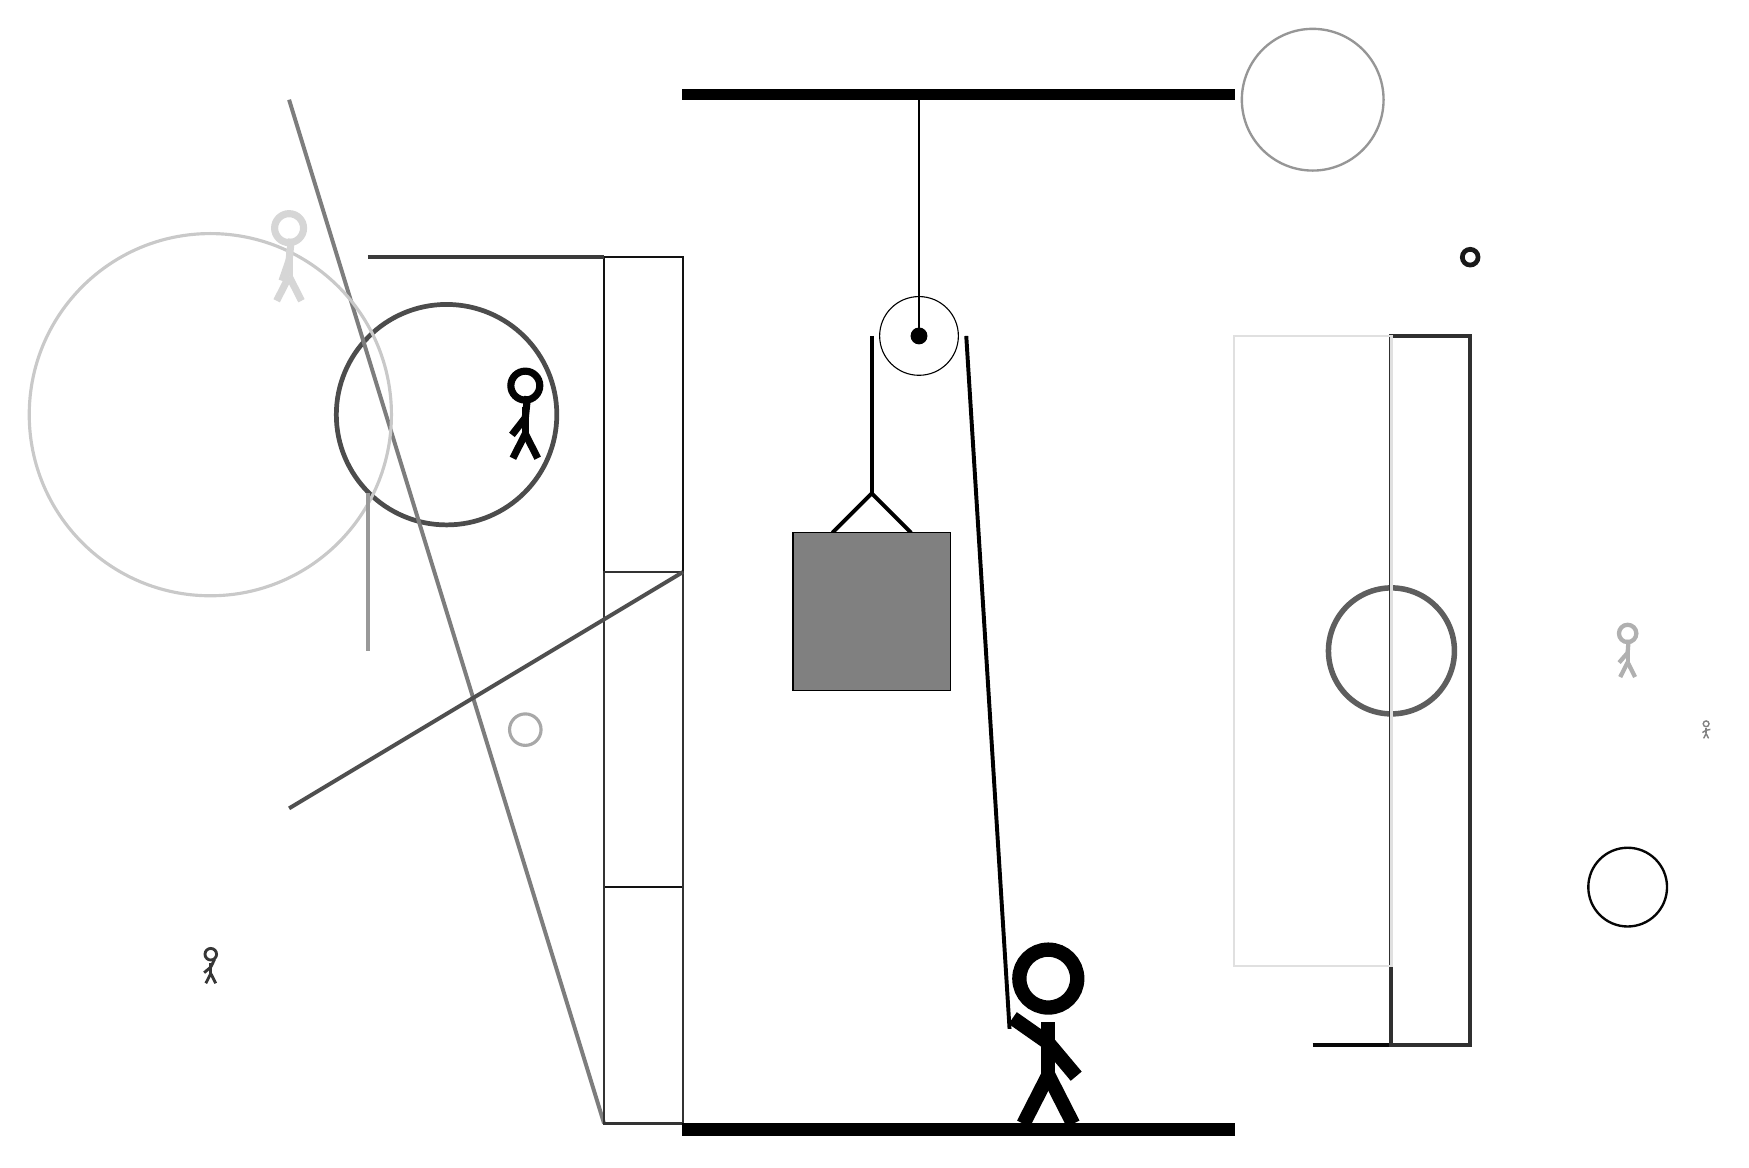
\begin{tikzpicture}
		%%%%% START %%%%%
		
		\draw[fill=black] (-2, 10) rectangle (5, 10.125);
		
		\draw (1, 7) circle (0.5);
		\draw[fill=black] (1, 7) circle (0.1);
		\draw (1, 10) -- (1, 7);
		
		\draw[line width=0.5mm] (-0.1, 4.5) -- (0.4, 5.0) -- (0.9, 4.5);
		\draw[fill=black!50] (-0.6, 4.5) rectangle (1.4, 2.5);
		
		\draw[line width=0.5mm] (0.4, 7) -- (0.4, 5.0);
		\centerarc[line width=0.5mm](1, 7)(0:180:0.6);
		\draw[line width=0.5mm](1.6, 7) -- (2.15, -1.8);
		
		\draw[line width=0.2mm, color=black!93] (-3, 8) rectangle (-2, 0);
		
		\draw [line width=0.6mm, color=black!70](-5, 6) circle (1.4);
		\draw [line width=0.6mm, color=black!90](8, 8) circle (0.1);
		\node[line width=0.3mm, color=black!31] at (10, 3) {\Strichmaxerl[3][49][86]};
		
		\draw[line width=0.5mm, color=black!51](-7, 10) -- (-3, -3);
		\node[line width=0.5mm, color=black!49] at (11, 2) {\Strichmaxerl[1][32][11]};
		
		\draw [line width=0.4mm, color=black!21](-8, 6) circle (2.3);
		\draw [line width=0.7mm, color=black!63](7, 3) circle (0.8);
		\draw[line width=0.3mm, color=black!80] (-3, 4) rectangle (-2, -3);
		
		\draw[line width=0.5mm, color=black!40](-6, 5) -- (-6, 3);
		
		\draw[line width=0.5mm, color=black!97](6, -2) -- (8, -2);
		\draw [line width=0.3mm, color=black!41](6, 10) circle (0.9);
		\node[line width=0.7mm, color=black!99] at (-4, 6) {\Strichmaxerl[5][52][84]};
		
		\node[line width=0.5mm, color=black!16] at (-7, 8) {\Strichmaxerl[5][71][84]};
		\draw[line width=0.5mm, color=black!69](-2, 4) -- (-7, 1);
		\draw [line width=0.3mm, color=black!98](10, 0) circle (0.5);
		
		\node[line width=0.3mm, color=black!79] at (-8, -1) {\Strichmaxerl[2][40][64]};
		
		\draw[line width=0.5mm, color=black!45] (7, 7) rectangle (7, 2);
		\draw[line width=0.5mm, color=black!77](-6, 8) -- (-3, 8);
		\draw[line width=0.5mm, color=black!81] (7, -2) rectangle (8, 7);
		\draw[line width=0.3mm, color=black!12] (5, -1) rectangle (7, 7);
		
		\draw [line width=0.4mm, color=black!34](-4, 2) circle (0.2);
		
		\node at (2.6, -1.9) {\Strichmaxerl[10][-35][-50]};
		
		\draw[fill=black] (-2, -3) rectangle (5, -3.15);
		
		%%%%% END %%%%%
	\end{tikzpicture}
\end{document}